

\tikzset{every picture/.style={line width=0.75pt}} %set default line width to 0.75pt        

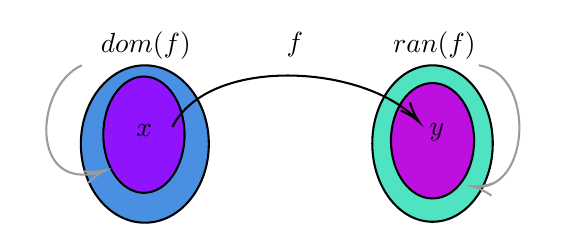
\begin{tikzpicture}[x=0.75pt,y=0.75pt,yscale=-1,xscale=1, scale=0.9]
%uncomment if require: \path (0,300); %set diagram left start at 0, and has height of 300

%Flowchart: Connector [id:dp590735645517438] 
\draw  [fill={rgb, 255:red, 74; green, 144; blue, 226 }  ,fill opacity=1 ] (51,94.13) .. controls (51,70.86) and (66.33,52) .. (85.25,52) .. controls (104.17,52) and (119.5,70.86) .. (119.5,94.13) .. controls (119.5,117.39) and (104.17,136.25) .. (85.25,136.25) .. controls (66.33,136.25) and (51,117.39) .. (51,94.13) -- cycle ;
%Flowchart: Connector [id:dp9948606826522155] 
\draw  [fill={rgb, 255:red, 80; green, 227; blue, 194 }  ,fill opacity=1 ] (207,93.88) .. controls (207,70.75) and (221.44,52) .. (239.25,52) .. controls (257.06,52) and (271.5,70.75) .. (271.5,93.88) .. controls (271.5,117) and (257.06,135.75) .. (239.25,135.75) .. controls (221.44,135.75) and (207,117) .. (207,93.88) -- cycle ;
%Shape: Ellipse [id:dp10431888056528327] 
\draw  [fill={rgb, 255:red, 144; green, 19; blue, 254 }  ,fill opacity=1 ] (63,89.13) .. controls (63,71.94) and (72.74,58) .. (84.75,58) .. controls (96.76,58) and (106.5,71.94) .. (106.5,89.13) .. controls (106.5,106.31) and (96.76,120.25) .. (84.75,120.25) .. controls (72.74,120.25) and (63,106.31) .. (63,89.13) -- cycle ;
%Shape: Ellipse [id:dp7464081859298852] 
\draw  [fill={rgb, 255:red, 189; green, 16; blue, 224 }  ,fill opacity=1 ] (217,92.38) .. controls (217,75.32) and (226.96,61.5) .. (239.25,61.5) .. controls (251.54,61.5) and (261.5,75.32) .. (261.5,92.38) .. controls (261.5,109.43) and (251.54,123.25) .. (239.25,123.25) .. controls (226.96,123.25) and (217,109.43) .. (217,92.38) -- cycle ;
%Curve Lines [id:da9031859390569301] 
\draw    (100,85) .. controls (119.21,46.83) and (201.96,51.11) .. (230.72,80.87) ;
\draw [shift={(232,82.25)}, rotate = 228.42] [color={rgb, 255:red, 0; green, 0; blue, 0 }  ][line width=0.75]    (10.93,-3.29) .. controls (6.95,-1.4) and (3.31,-0.3) .. (0,0) .. controls (3.31,0.3) and (6.95,1.4) .. (10.93,3.29)   ;
%Curve Lines [id:da4731770474888055] 
\draw [color={rgb, 255:red, 155; green, 155; blue, 155 }  ,draw opacity=1 ]   (51.5,52) .. controls (25.89,63.57) and (23.08,120.99) .. (62.18,108.85) ;
\draw [shift={(64,108.25)}, rotate = 160.52] [color={rgb, 255:red, 155; green, 155; blue, 155 }  ,draw opacity=1 ][line width=0.75]    (10.93,-3.29) .. controls (6.95,-1.4) and (3.31,-0.3) .. (0,0) .. controls (3.31,0.3) and (6.95,1.4) .. (10.93,3.29)   ;
%Curve Lines [id:da15941181414201] 
\draw [color={rgb, 255:red, 155; green, 155; blue, 155 }  ,draw opacity=1 ]   (264,52) .. controls (294.38,56.17) and (292.11,119.15) .. (262.36,116.97) ;
\draw [shift={(260.5,116.75)}, rotate = 9.02] [color={rgb, 255:red, 155; green, 155; blue, 155 }  ,draw opacity=1 ][line width=0.75]    (10.93,-3.29) .. controls (6.95,-1.4) and (3.31,-0.3) .. (0,0) .. controls (3.31,0.3) and (6.95,1.4) .. (10.93,3.29)   ;

% Text Node
\draw (79,81.9) node [anchor=north west][inner sep=0.75pt]    {$x$};
% Text Node
\draw (236,81.4) node [anchor=north west][inner sep=0.75pt]  [color={rgb, 255:red, 0; green, 0; blue, 0 }  ,opacity=1 ]  {$y$};
% Text Node
\draw (159.5,32.4) node [anchor=north west][inner sep=0.75pt]    {$f$};
% Text Node
\draw (60,32.4) node [anchor=north west][inner sep=0.75pt]    {$\operatorname{dom}( f)$};
% Text Node
\draw (216.5,32.4) node [anchor=north west][inner sep=0.75pt]    {$\operatorname{ran}( f)$};


\end{tikzpicture}
